\chapter{Synthetic Dataset Generation}

\par The aim of generating this dataset was to challenge the existing detection scheme. Image properties between ham and spam images vary. We used Image Processing techniques on spam images, to make it look more like a ham image. A public corpus; Spam Archive, from Dredze et. al in their paper Learning Fast Classifiers~\cite{10} included only spam images. We used this corpus and overlayed it on the ham images from Dataset 1. The resulting spam images were harder to detect.


\par There are two key steps to generating this test dataset- 
\begin{itemize}
	\item First, we resize the spam image to the dimensions of ham image. This resizing helps align the file properties of the test dataset to that of ham set.
	
	\item Second, we overlay spam images on top of ham images. A general observation we made with the spam images, was that spam images have a light (white/yellow) background. Eliminating the background, we picked up only the content of the spam image and overlaid it on ham image. Doing so, helped us align many image properties like color histogram and edges with that of ham images.
	
\end{itemize}

\par Fig. \ref{fig:testDataset}. shows an example of the generated dataset. We can see that the test image(generated image), has the ham image as the background and the content of the spam image as the foreground. 

\begin{figure}[htb]
	\centering
	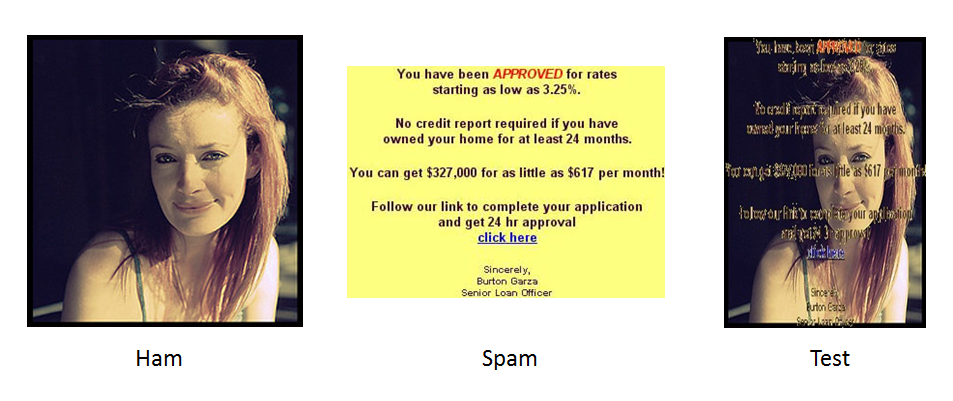
\includegraphics[scale=0.7]{images/testDataset.PNG}
	\caption{Test dataset example}
	\label{fig:testDataset}
\end{figure} 

\par Fig. \ref{fig:Scatter_Plots}. shows scatterplots of compression ratio and color entropy values for ham, spam and test images. It is easy to note from these scatterplots how the properties of ham and test image align. Appendix \ref{app:a} lists scatter plots of rest of the features.

 \begin{figure}[h]
 	
 	\begin{subfigure}{0.5\textwidth}
 		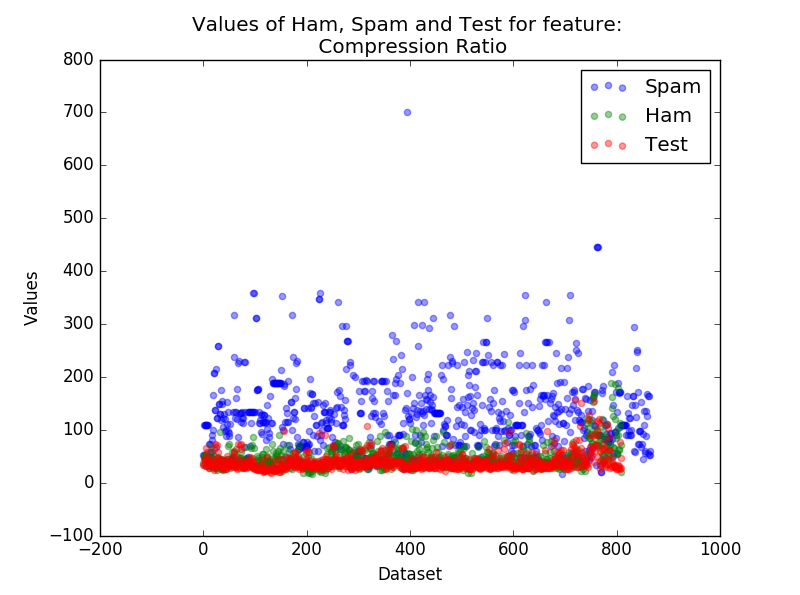
\includegraphics[width=0.9\linewidth]{images/CompressionRatio_values_scatter} 
 		\caption{Compression Ratio}
 		\label{fig:AUC_Dataset1_linear}
 	\end{subfigure}
 	\begin{subfigure}{0.5\textwidth}
 		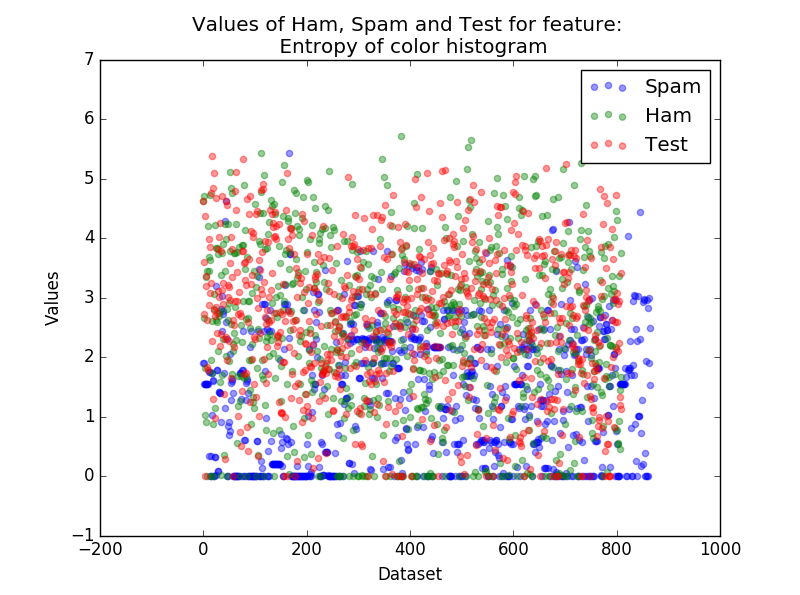
\includegraphics[width=0.9\linewidth]{images/EntropyOfColorHistogram_values_scatter}
 		\caption{Entropy of color histogram}
 		\label{fig:CM_Dataset1_linear}
 	\end{subfigure}
 	
 	\caption{Feature value comparison scatter plots}
 	\label{fig:Scatter_Plots}
 \end{figure}
 





